\documentclass[t]{beamer}
\usepackage{helvet}
\usepackage{calc}
\usepackage[utf8]{inputenc} % set your input encoding differently, if you want
\usepackage[english]{babel}

% Setting style of presentation
% =============================
\usetheme{Boadilla}
%\setbeamercovered{transparent=10}
%\setbeamertemplate{navigation symbols}{}


% Some common packages
% ====================
\usepackage{units}
\usepackage{amsbsy}
\usepackage{amsmath}
\usepackage{amssymb}
\usepackage{graphics}
\usepackage{epsf}
\usepackage{epsfig}
\usepackage{fixmath}
\usepackage{wrapfig}
\usepackage{tcolorbox}

\usepackage{array}
\newcolumntype{M}{>{\centering\arraybackslash}m{\dimexpr.25\linewidth-2\tabcolsep}}

% Adapt title information
% =======================
\title{Development of a temperature sensor network\\for the nEDM experiment}
\author{Wenwen Chen, Rainer Schönberger}
%\institute{Department for Computer Science\\Technische Universität München}
\date{\today}





% ==============
% DOCUMENT BEGIN
% ==============
\begin{document}

% Typeset title page
% ------------------------------------------------------------------------
%\setbeamertemplate{background}{\NETBlackTransparent{width=2.3\paperwidth}}
\begin{frame}
    \titlepage
\end{frame}
%\setbeamertemplate{background}{}
% ------------------------------------------------------------------------

% Outline
% ------------------------------------------------------------------------
%\begin{frame}
%    \frametitle{Outline}
%    \tableofcontents
%\end{frame}
% ------------------------------------------------------------------------



% MOTIVATION
% ------------------------------------------------------------------------
\begin{frame}[c]
    \frametitle{Requirements}
		\begin{alertblock}{High priority}
			\begin{itemize}
				\item High numer of sensors: 48
				\item As accurate as possible:  $\pm0.1\mathrm{K}$
				\item Support for temperature and humidity sensors
				\item Send results to couchDB
			\end{itemize}
		\end{alertblock}
		\begin{exampleblock}{Low priority}
			\begin{itemize}
				\item Extendable
				\item Plug and Play
				\item Sample interval $\le 1\mathrm{s}$
				\item Easy configuration at runtime
			\end{itemize}
		\end{exampleblock}
\end{frame}
\begin{frame}[c]
    \frametitle{Sensor comparison}
\begin{tabular}{ M M M M}
	Sensor & Accuracy & Resolution & Cost\tabularnewline
	\hline
	\hline
	TSIC 506F& $\pm 0.1\mathrm{K}$ & $\pm 0.034\mathrm{K}$ & $8 \mathrm{EUR}$\tabularnewline
	\hline
	HYT271 (humidity)& $\pm 1.8\mathrm{\%RH}$ & $\pm 0.03\mathrm{\%RH}$ & $20 \mathrm{EUR}$\tabularnewline
	HYT271 (temperature)& $\pm 0.2\mathrm{K}$ & $\pm 0.015\mathrm{K}$ & $20 \mathrm{EUR}$\tabularnewline
	\hline
\end{tabular}
\end{frame}
\begin{frame}[c]
    \frametitle{Logical structure}
  \begin{center}
  	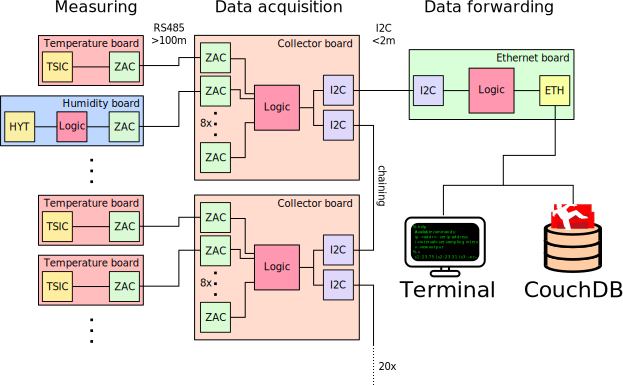
\includegraphics[width=0.9\linewidth]{img/plan2_color.pdf}\\
  \vspace{0.5cm}
  \end{center}
    
\end{frame}
\begin{frame}[c]
    \frametitle{Proof of concept}
  \begin{center}
  	\includegraphics[width=0.8\linewidth]{img/pic/IMG_20140410_213954.jpg}\\
  \vspace{0.5cm}
  \end{center}
\end{frame}
\begin{frame}[c]
    \frametitle{First load of PCBs arrived}
  \begin{center}
  	\includegraphics[width=0.8\linewidth]{img/pic/platinen_leer.jpg}\\
  \vspace{0.5cm}
  \end{center}
\end{frame}
\begin{frame}[c]
    \frametitle{Hours of soldering later...}
  \begin{center}
  	\includegraphics[width=0.8\linewidth]{img/pic/platinen_geloetet.jpg}\\
  \vspace{0.5cm}
  \end{center}
\end{frame}
\begin{frame}[c]
    \frametitle{Collector board}
  \begin{center}
  	\includegraphics[width=0.4\linewidth]{img/pic/collector_geloetet.jpg}\\
  \vspace{0.5cm}
  \end{center}
\end{frame}
\begin{frame}[c]
    \frametitle{3D - Printing}
  \begin{center}
  	\includegraphics[width=0.8\linewidth]{img/pic/IMG_20140530_184940.jpg}\\
  \vspace{0.5cm}
  \end{center}
\end{frame}
\begin{frame}[c]
    \frametitle{Finished cases}
  \begin{center}
  	\includegraphics[width=0.9\linewidth]{img/pic/cases.jpg}\\
  \vspace{0.5cm}
  \end{center}
\end{frame}
\end{document}
